\documentclass[10pt,a5paper]{article}
\usepackage{graphicx}
\usepackage{hyperref}
\usepackage[utf8x]{inputenc}

\begin{document}

\begin{titlepage}
\begin{center}

\huge
Ninetails

Quick Start Manual

\vspace*{2cm}

\normalsize
Low cost, high performance accelerator for Amiga 600.

\vspace*{2cm}
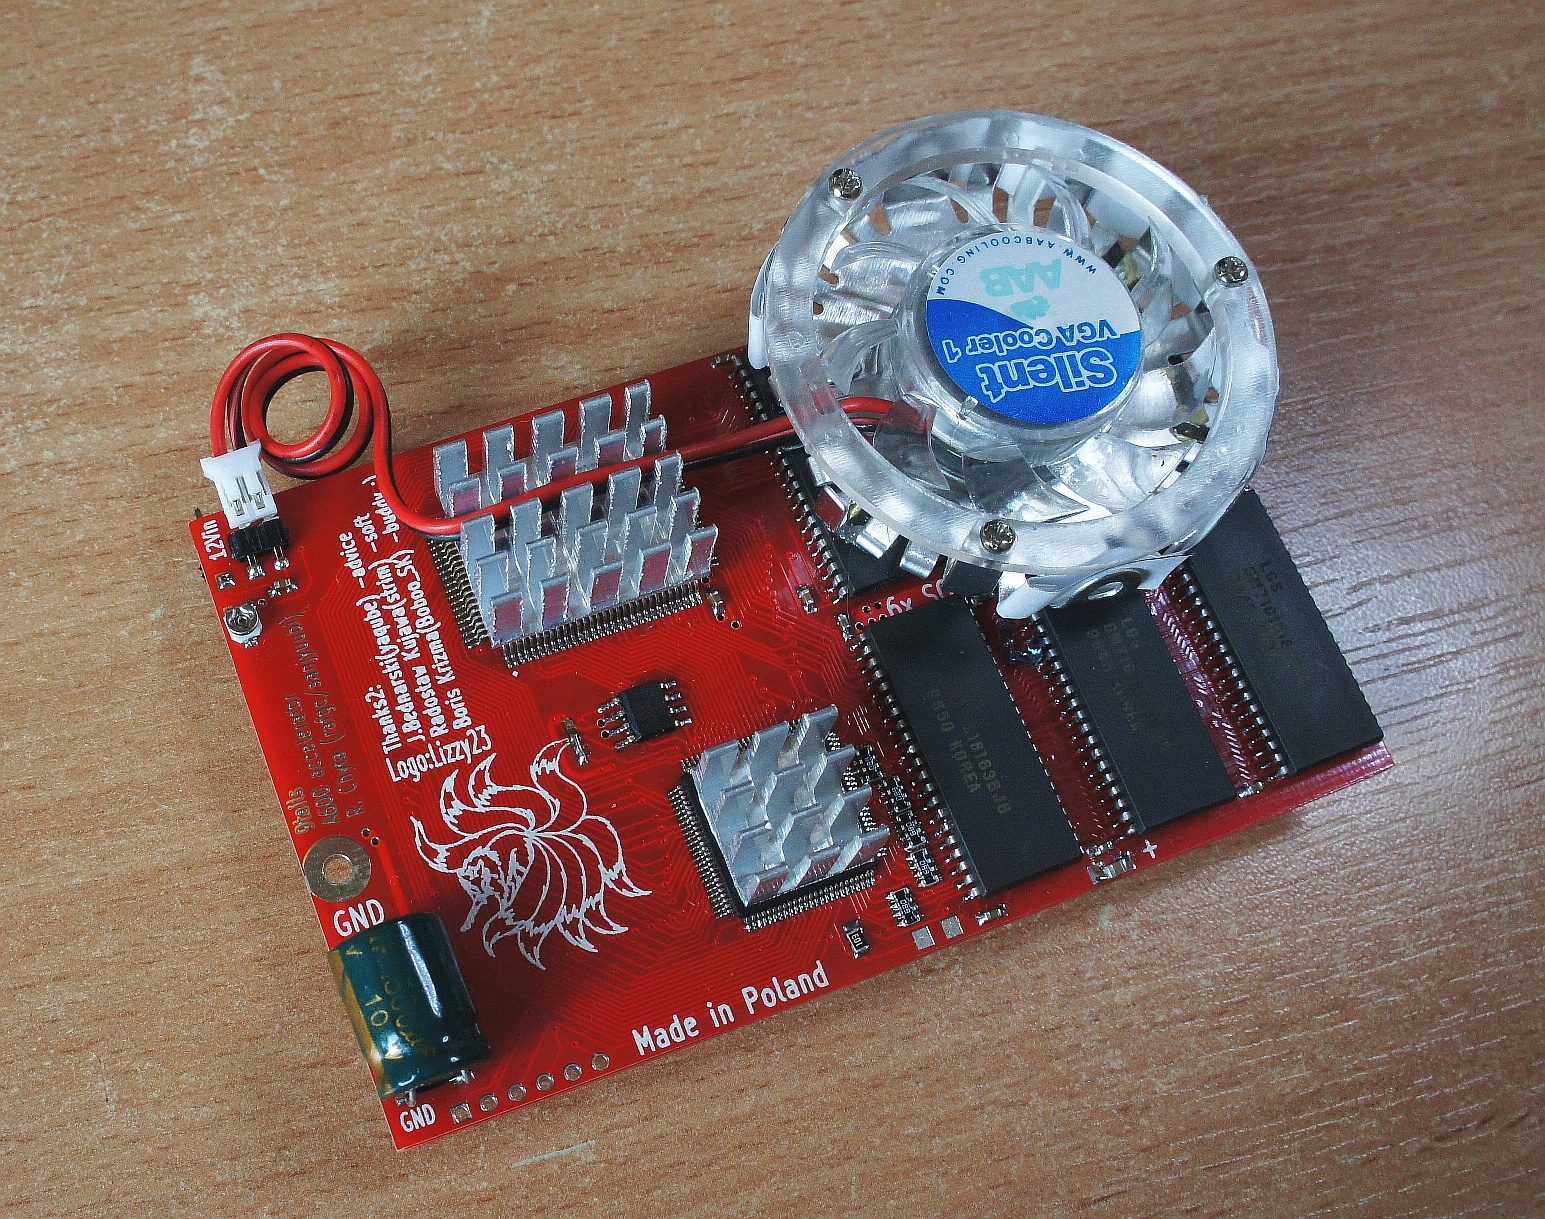
\includegraphics[scale=0.15]{ninetails-photo.jpg}
\vfill

\normalsize
\today

\end{center}
\end{titlepage}

\section*{Overview}

Thank you for purchasing Ninetails accelerator. It has several advanced features:

\begin{itemize}
	\item 28MHz MC68EC020 processor.
	\item Total of 11MB RAM accessible from operating system -- 8MB auto configuring Fast RAM, 1.5MB Slow RAM, 1.5MB additional Fast RAM.
	\item Shadow ROM and MAPROM functions.
	\item Optional PCMCIA compatibility mode (reduces auto configuring Fast RAM to 4 MB).
	\item Ability to disable the card through software (no need to install physical switch).
\end{itemize}

\begin{center}
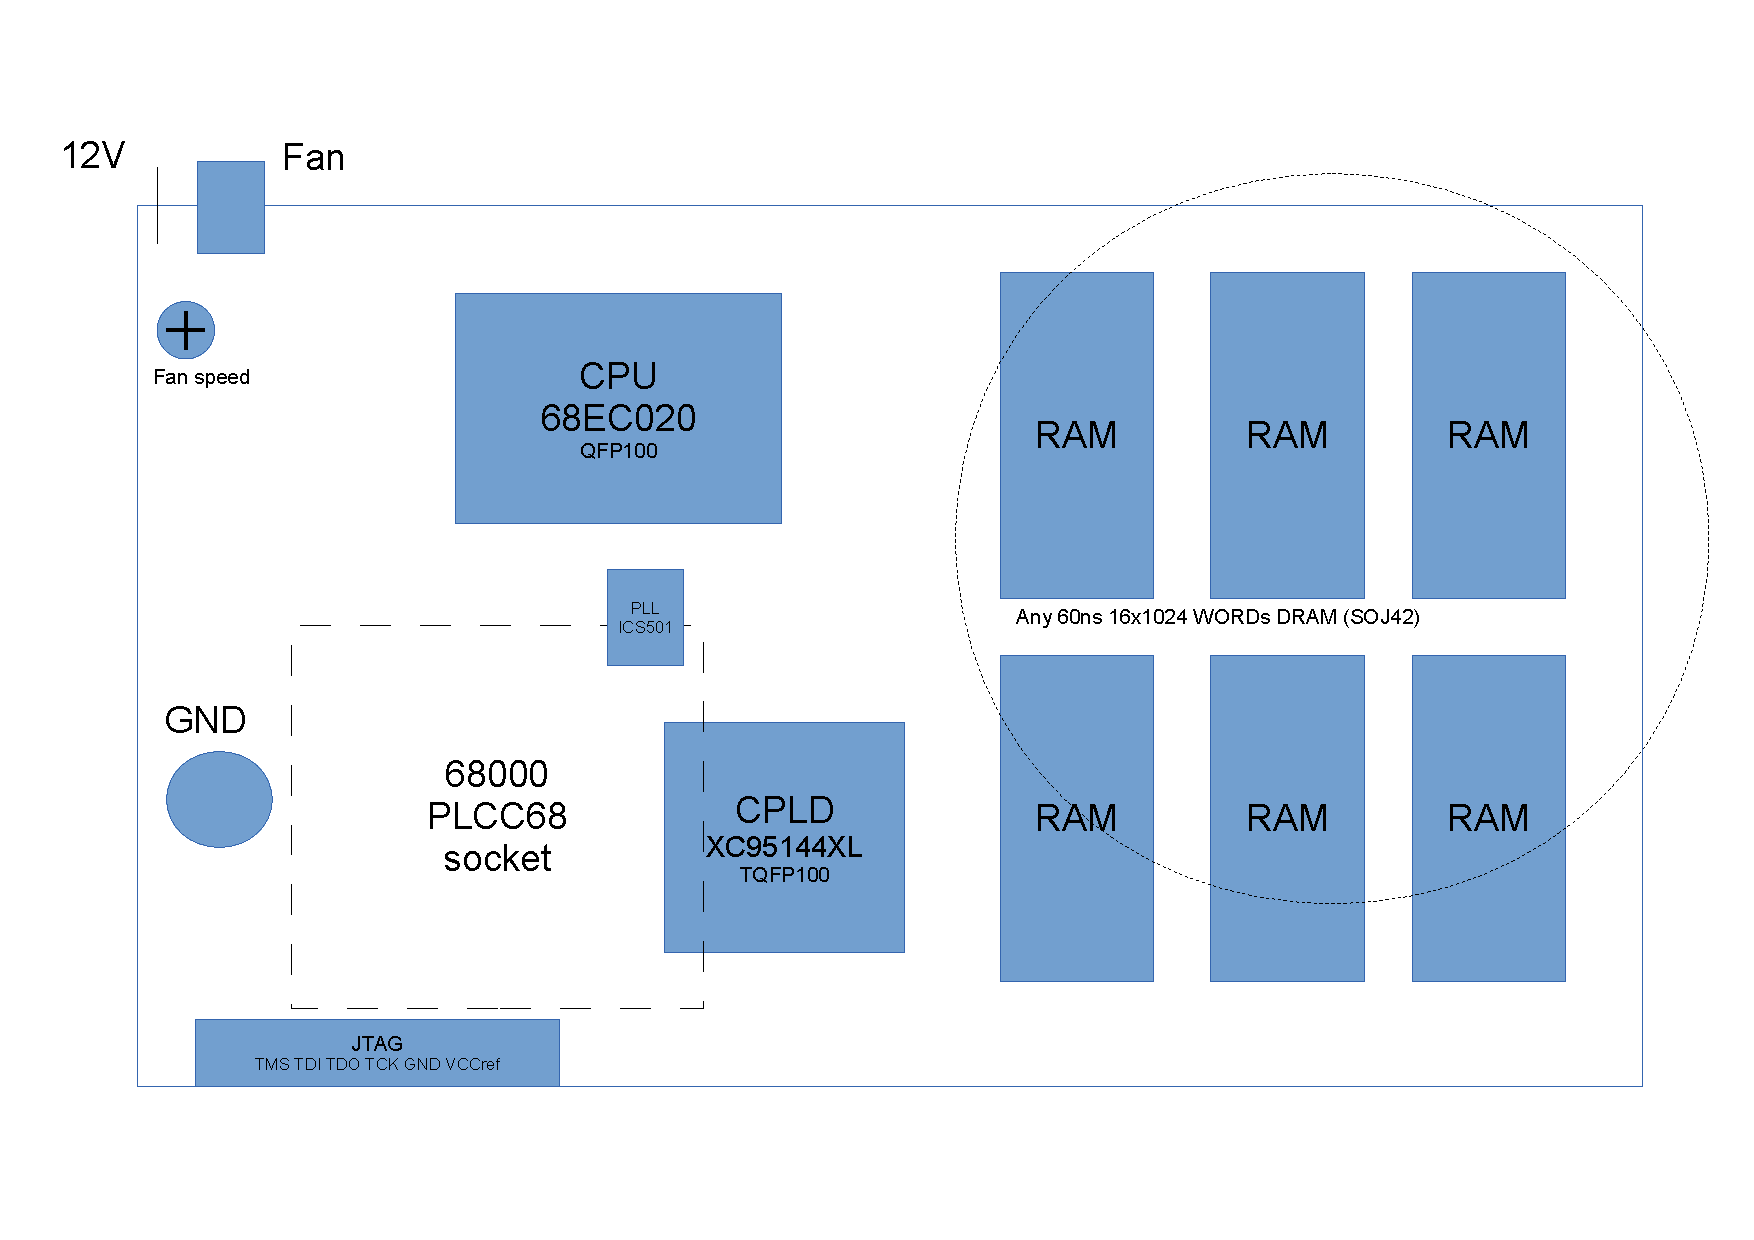
\includegraphics[scale=0.25]{ninetails-drawing.pdf}
\end{center}

Due to space restrictions, Ninetails is not compatible with standard Amiga 600 hard disk mounting cradle. It is advised to use Compact Flash instead of hard disk. 

The card produces some amount of heat. Do not modify the original cooling devices.

\section*{Installation}

The installation process is not complicated, but should be performed carefully. Your Ninetails package should contain the following items:

\begin{itemize}
	\item Ninetails accelerator board.
	\item 12V jumper wire.
	\item Small screw and sleeve.
	\item This manual.
\end{itemize}

To install Nintetails in the Amiga perform the following steps:

\begin{itemize}
	\item Open your Amiga 600.
	\item Place Ninetails board PLCC socket on top of 68000 processor and press gently. 12V connector should be pointing towards the back of the Amiga (where ports are located).
	\item Connect 12V input on Ninetails with appropriate pin on the power connector, using attached wire.
	\item Insert the sleeve under GND through hole (bottom left part of the PCB) and screw the hole to Amiga main board.
	\item Close your Amiga.
\end{itemize}

Your Amiga should start as normal, albeit much faster. After installation you can confirm that the board is working correctly, by checking type of processor with the {\tt cpu} command and amount of memory with the {\tt avail} command.

To use advanced features of the accelerator install the {\tt 9tcfg} utility. It can be downloaded from \url{http://...}. Source code is available through the GitHub repository: \url{http://github.com/rkujawa/9tcfg/}. Read the attached documentation for more information on how to use it. 

\section*{Acknowledgements}

The Ninetails board was designed and produced by Rafał ,,rafgc'' Chyła. 9tcfg program and this manual were written by Radosław ,,strim'' Kujawa.

Thanks are going to the following people: Jakub ,,yaqube'' Bednarski, Boris ,,Boboo\_SK'' Krizma. Ninetails logo was done by Lizzy23.

\end{document}
